\documentclass[aspectratio=169,10pt]{beamer}

\usepackage[T1]{fontenc}
\usepackage[utf8]{inputenc}
\usepackage[scaled=.96]{helvet}
\renewcommand{\familydefault}{\sfdefault}
\usepackage{booktabs}
\usepackage{listings}
\usepackage{tikz}
\usetikzlibrary{arrows.meta,positioning,shapes.geometric}

% Colours and typography follow the restrained IETF 124 slide deck.
\definecolor{ietfteal}{HTML}{003B49}
\definecolor{ietfblue}{HTML}{176B87}
\definecolor{ietfnavy}{HTML}{003B49}
\definecolor{lightblue}{HTML}{EAF2F4}
\definecolor{softgray}{HTML}{F4F4F4}
\definecolor{darkgray}{HTML}{444444}
\definecolor{pagenumbergray}{HTML}{8C8C8C}
\definecolor{accent}{HTML}{D95F02}
\definecolor{good}{HTML}{2B7A3D}

\setbeamercolor{normal text}{fg=black,bg=white}
\setbeamercolor{structure}{fg=black}
\setbeamercolor{frametitle}{fg=black,bg=white}
\setbeamercolor{title}{fg=white}
\setbeamercolor{subtitle}{fg=lightblue}
\setbeamercolor{author}{fg=white}
\setbeamercolor{date}{fg=lightblue}
\setbeamercolor{block title}{fg=black,bg=softgray}
\setbeamercolor{block body}{fg=black,bg=softgray}
\setbeamercolor{alerted text}{fg=accent}
\setbeamercolor{footline}{fg=pagenumbergray,bg=white}

\setbeamerfont{frametitle}{size=\LARGE,series=\mdseries}
\setbeamerfont{block title}{series=\bfseries}
\setbeamersize{text margin left=.9cm,text margin right=.9cm}

\setbeamertemplate{navigation symbols}{}
\setbeamertemplate{itemize item}{\raise0.1ex\hbox{\small$\bullet$}}
\setbeamertemplate{itemize subitem}{\raise0.1ex\hbox{\scriptsize$\bullet$}}
\setbeamertemplate{footline}{
  \leavevmode%
  \begin{beamercolorbox}[wd=\paperwidth,ht=2.5ex,dp=1.2ex,rightskip=.85cm]{footline}%
    \hfill\insertframenumber
  \end{beamercolorbox}%
}
\setbeamertemplate{frametitle}{
  \nointerlineskip
  \begin{beamercolorbox}[wd=\paperwidth,ht=3.1ex,dp=.85ex,leftskip=.9cm,rightskip=.9cm]{frametitle}
    \usebeamerfont{frametitle}\insertframetitle
  \end{beamercolorbox}
}

\newcommand{\field}[2]{%
  \begin{tikzpicture}[baseline=(n.base)]
    \node[rounded corners=2pt,fill=#1,inner xsep=5pt,inner ysep=2pt,text=white,font=\scriptsize\bfseries] (n) {#2};
  \end{tikzpicture}%
}
\newcommand{\yes}{\textcolor{good}{\bfseries Yes}}
\newcommand{\changed}{\textcolor{accent}{\bfseries Changed}}

\lstdefinestyle{json}{
  basicstyle=\ttfamily\fontsize{6.7}{7.5}\selectfont,
  columns=fullflexible,
  keepspaces=true,
  showstringspaces=false,
  frame=single,
  rulecolor=\color{ietfblue},
  backgroundcolor=\color{softgray},
  xleftmargin=3pt,
  xrightmargin=3pt,
  framexleftmargin=2pt,
  framexrightmargin=2pt,
  aboveskip=3pt,
  belowskip=2pt
}

\title{Requesting a Freshness Nonce for\\Attestation Evidence in CSRs}
\subtitle{What changed from draft-ietf-lamps-attestation-freshness -05 to -08}
\author{Hannes Tschofenig, Hendrik Brockhaus, Joe Mandel, Sean Turner}
\date{IETF LAMPS Working Group, IETF 126, July 2026}

\begin{document}

{
\setbeamercolor{background canvas}{bg=white}
\begin{frame}[plain]
  % Dark upper field and white logo band as in ietf124_slides_lamps.pdf.
  \begin{tikzpicture}[remember picture,overlay]
    \fill[ietfteal]
      (current page.north west) rectangle
      ([yshift=-.80\paperheight]current page.north east);
    \node[anchor=south east,inner sep=0pt]
      at ([xshift=-.72cm,yshift=.23cm]current page.south east)
      {\IfFileExists{ietf-logo.png}
        {
\includegraphics[width=2.15cm]{ietf-logo.png}}
        {\color{ietfteal}\fontsize{22}{22}\selectfont\bfseries ietf}};
  \end{tikzpicture}

  \vspace{.28cm}
  {\color{white}\fontsize{24}{27}\selectfont\bfseries\inserttitle\par}
  \vspace{.14cm}
  {\color{white}\fontsize{12}{14}\selectfont\bfseries\insertsubtitle\par}
  \vspace{.55cm}
  {\color{white}\fontsize{10.5}{12}\selectfont\insertauthor\par}
  \vfill
  {\color{white}\fontsize{12}{14}\selectfont\bfseries\insertdate\par}
  \vspace{.12cm}
  {\color{white}\footnotesize -05: 19 October 2025 \hspace{0.7em}$\longrightarrow$\hspace{0.7em} -08: 4 July 2026}
  \vspace{1.12cm}
\end{frame}
}

\begin{frame}{Why the larger update now?}
  \begin{columns}[T,onlytextwidth]
    \begin{column}{0.55\textwidth}
      \begin{block}{A direct dependency}
        This document defines freshness for Evidence carried using
        \texttt{draft-ietf-lamps-csr-attestation}.
      \end{block}
      \vspace{0.2cm}
      The CSR Attestation draft made \alert{significant progress earlier this year}.  That provided a firmer basis for:
      \begin{itemize}
        \item the architecture and terminology,
        \item the relation between a nonce and Evidence, and
        \item support for multiple Attesters and Evidence statements.
      \end{itemize}
    \end{column}
    \begin{column}{0.40\textwidth}
      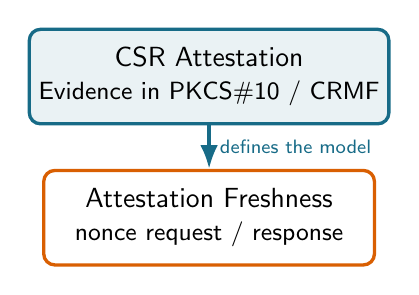
\begin{tikzpicture}[node distance=0.55cm, every node/.style={align=center}]
        \node[draw=ietfblue,very thick,rounded corners,fill=lightblue,
              minimum width=4.2cm,minimum height=1.2cm] (csr)
              {CSR Attestation\\\small Evidence in PKCS\#10 / CRMF};
        \node[draw=accent,very thick,rounded corners,fill=white,
              minimum width=4.2cm,minimum height=1.2cm,below=of csr] (fresh)
              {Attestation Freshness\\\small nonce request / response};
        \draw[-{Latex[length=3mm]},very thick,ietfblue] (csr) -- node[right,font=\scriptsize]{defines the model} (fresh);
      \end{tikzpicture}
      \vspace{0.25cm}

      \centering\small The -08 changes align the two drafts.
    \end{column}
  \end{columns}
\end{frame}

\begin{frame}{Changes from -05 to -08}
  \begin{columns}[T,onlytextwidth]
    \begin{column}{0.47\textwidth}
      \textbf{\color{darkgray}-05}
      \vspace{0.12cm}
      \begin{itemize}
        \item ``Conveying a nonce'' separately in CMP, EST, and CMC
        \item Arrays / sequences of nonce requests
        \item \texttt{type} and free-form \texttt{hint} tied to a Verifier
        \item Protocol-specific structures evolved independently
      \end{itemize}
    \end{column}
    \begin{column}{0.06\textwidth}
      \centering\vspace{1.3cm}
      {\color{accent}\Large$\Longrightarrow$}
    \end{column}
    \begin{column}{0.47\textwidth}
      \textbf{\color{ietfblue}-08}
      \vspace{0.12cm}
      \begin{itemize}
        \item One common architecture and message model
        \item One nonce request and one nonce response
        \item Typed, extensible \texttt{reqInfo} / \texttt{respInfo}
        \item Consistent ASN.1 and CDDL representations
        \item Protocol bindings are separate from message semantics
      \end{itemize}
    \end{column}
  \end{columns}
  \vspace{0.25cm}
  \begin{block}{Scope}
    Request a nonce before enrollment; include it only inside the attestation
    Evidence carried by the subsequent CSR.
  \end{block}
\end{frame}

\begin{frame}{Architecture}
  \centering
  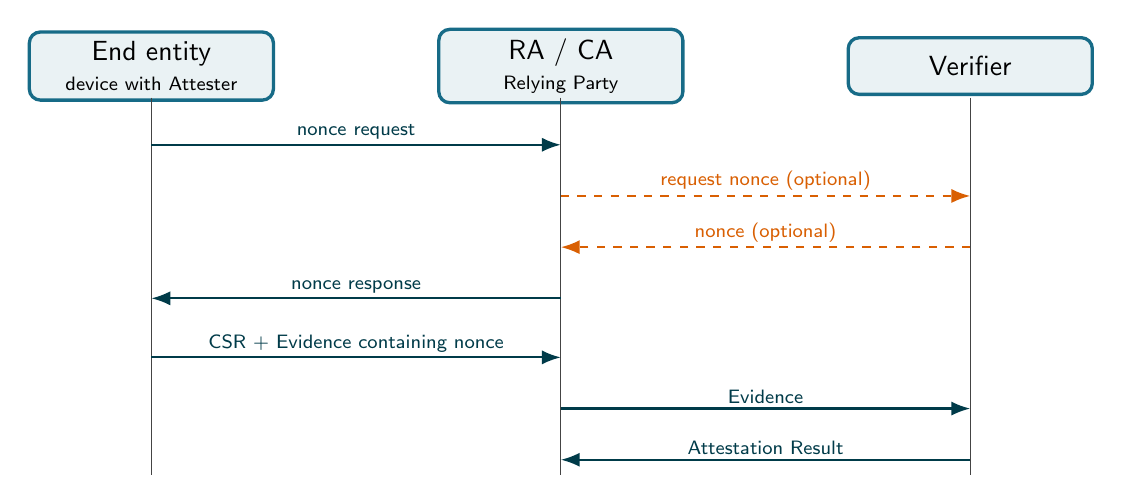
\begin{tikzpicture}[
    x=1cm,y=1cm,
    actor/.style={draw=ietfblue,very thick,rounded corners,fill=lightblue,
                  minimum width=3.1cm,minimum height=.72cm,align=center},
    msg/.style={-{Latex[length=2.4mm]},thick,ietfnavy},
    opt/.style={-{Latex[length=2.4mm]},thick,dashed,accent},
    label/.style={font=\scriptsize,fill=white,inner sep=1.5pt}
  ]
    \node[actor] (ee) at (0,0) {End entity\\[-1pt]\scriptsize device with Attester};
    \node[actor] (ra) at (5.2,0) {RA / CA\\[-1pt]\scriptsize Relying Party};
    \node[actor] (v)  at (10.4,0) {Verifier};
    \draw[darkgray] (0,-.4) -- (0,-5.2);
    \draw[darkgray] (5.2,-.4) -- (5.2,-5.2);
    \draw[darkgray] (10.4,-.4) -- (10.4,-5.2);

    \draw[msg] (0,-1.0) -- node[label,above]{nonce request} (5.2,-1.0);
    \draw[opt] (5.2,-1.65) -- node[label,above]{request nonce (optional)} (10.4,-1.65);
    \draw[opt] (10.4,-2.3) -- node[label,above]{nonce (optional)} (5.2,-2.3);
    \draw[msg] (5.2,-2.95) -- node[label,above]{nonce response} (0,-2.95);
    \draw[msg] (0,-3.7) -- node[label,above]{CSR + Evidence containing nonce} (5.2,-3.7);
    \draw[msg] (5.2,-4.35) -- node[label,above]{Evidence} (10.4,-4.35);
    \draw[msg] (10.4,-5.0) -- node[label,above]{Attestation Result} (5.2,-5.0);
  \end{tikzpicture}

  \vspace{0.08cm}
  \small
  \textbf{In scope:} the interface between the End Entity and the Relying Party
  (RA/CA). \textbf{Out of scope:} the interface between the Relying Party and
  the Verifier.
\end{frame}

\begin{frame}{Freshness: nonce vs. claim data}
  \footnotesize
  \begin{columns}[T,onlytextwidth]
    \begin{column}{0.47\textwidth}
      \begin{block}{Nonce-based freshness}
        \begin{itemize}
          \setlength{\itemsep}{2pt}
          \item The RP or Verifier provides an unpredictable challenge;
                the Attester binds it to the Claims in protected Evidence.
          \item A match proves that the Evidence was produced after the
                challenge.
          \item An extra exchange and typically per-nonce state are required.
        \end{itemize}
        \vspace{0.08cm}
        \textcolor{good}{\bfseries In scope:} This document specifies the
        nonce exchange.
      \end{block}
    \end{column}
    \begin{column}{0.47\textwidth}
      \begin{block}{Freshness data in Claims}
        \begin{itemize}
          \setlength{\itemsep}{2pt}
          \item The time when the Claim values were collected by the
                Attesting Environment is, in general, unknown.
          \item Claim values may have changed between their collection and the
                production of the Evidence.
          \item Freshly signed Evidence does not by itself prove that individual Claim
                values were freshly collected.
        \end{itemize}
        \vspace{0.08cm}
        \textcolor{accent}{\bfseries Out of scope:} This document neither
        defines nor evaluates freshness data in Claims.
      \end{block}
    \end{column}
  \end{columns}
  \vspace{0.08cm}
  \begin{center}
    \alert{\bfseries Nonce freshness of Evidence $\neq$ freshness of individual Claim values.}
  \end{center}
\end{frame}

\begin{frame}{Extensibility}
  \begin{columns}[T,onlytextwidth]
    \begin{column}{0.47\textwidth}
      \begin{block}{NonceRequest}
        \field{ietfblue}{len}\quad optional, 8--64 bytes

        \vspace{0.25cm}
        \field{ietfblue}{reqTypeInfo}\quad optional
        \begin{itemize}
          \item \texttt{type}: OID identifying the syntax
          \item \texttt{reqInfo}: type-specific input
        \end{itemize}
      \end{block}
    \end{column}
    \begin{column}{0.47\textwidth}
      \begin{block}{NonceResponse}
        \field{accent}{nonce}\quad required, 0 or 8--64 bytes

        \vspace{0.16cm}
        \field{accent}{expiry}\quad optional, seconds

        \vspace{0.16cm}
        \field{accent}{respTypeInfo}\quad optional
        \begin{itemize}
          \item \texttt{type}: OID identifying the syntax
          \item \texttt{respInfo}: type-specific output
        \end{itemize}
      \end{block}
    \end{column}
  \end{columns}
  \vspace{0.25cm}
  \begin{center}
    \field{ietfnavy}{ASN.1 for CMP / CMC}
    \hspace{1.2cm}
    \field{good}{CDDL for EST JSON / CBOR}
  \end{center}
  \small\centering
  \texttt{reqInfo} and \texttt{respInfo} are defined by external, OID-identified profiles.
\end{frame}

\begin{frame}{Protocol bindings are aligned}
  \small
  \begin{tabular}{@{}p{1.4cm}p{3.1cm}p{3.0cm}p{4.9cm}@{}}
    \toprule
    \textbf{Protocol} & \textbf{Transport mechanism} & \textbf{Encoding} & \textbf{Notable -08 detail}\\
    \midrule
    CMP &
      \texttt{genm} / \texttt{genp} &
      ASN.1 &
      New information types; HTTP \texttt{getnonce} and CoAP \texttt{nonce} paths\\[0.2cm]
    EST over HTTPS &
      \texttt{GET} or \texttt{POST} on \texttt{/nonce} &
      JSON &
      Dedicated \texttt{application/est-}\newline
      \texttt{attestation-freshness+json} media type\\[0.2cm]
    EST over CoAPs &
      \texttt{GET} or \texttt{POST} on \texttt{/nonce} &
      CBOR &
      CoAP response codes and a dedicated CBOR media type / Content-Format\\[0.2cm]
    CMC &
      Controls in Full PKI Request &
      ASN.1 &
      Separate request / response control OIDs and explicit status handling\\
    \bottomrule
  \end{tabular}

  \vspace{0.35cm}
  \begin{center}
    \alert{\bfseries Same semantics across CMP, EST, and CMC; only the binding changes.}
  \end{center}
\end{frame}

\begin{frame}{EST is no longer an open design point}
  \begin{columns}[T,onlytextwidth]
    \begin{column}{0.46\textwidth}
      \textbf{\color{darkgray}-05}
      \begin{itemize}
        \item HTTPS + generic \texttt{application/json}
        \item JSON arrays and index-based correlation
        \item Absolute timestamp for \texttt{expiry}
        \item EST-over-CoAP / CBOR left as an open issue
      \end{itemize}
    \end{column}
    \begin{column}{0.50\textwidth}
      \textbf{\color{ietfblue}-08}
      \begin{itemize}
        \item HTTPS/JSON and secure CoAP/CBOR specified
        \item CDDL defines both representations
        \item One object; no positional correlation
        \item \texttt{expiry} consistently means validity in seconds
        \item Explicit success and error response codes
        \item Dedicated JSON and CBOR media types
      \end{itemize}
    \end{column}
  \end{columns}
  \vspace{0.3cm}
  \begin{block}{GET versus POST}
    \texttt{GET} when no optional request content is needed; \texttt{POST} when
    \texttt{len} or type-specific request information is conveyed.
  \end{block}
\end{frame}

\begin{frame}{Multiple Attesters}
  \begin{columns}[T,onlytextwidth]
    \begin{column}{0.52\textwidth}
      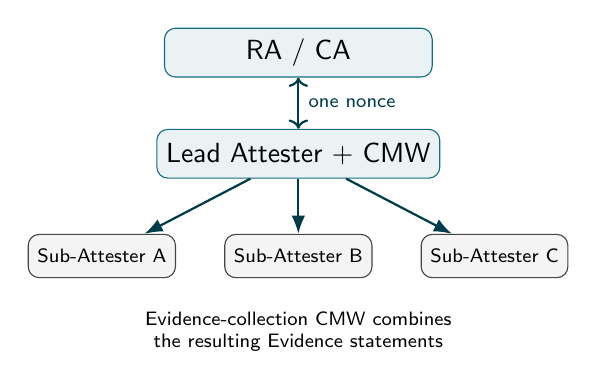
\begin{tikzpicture}[
        node distance=.35cm,
        box/.style={draw=ietfblue,rounded corners,fill=lightblue,
                    minimum width=3.4cm,minimum height=.62cm,align=center},
        sub/.style={draw=darkgray,rounded corners,fill=softgray,font=\scriptsize,
                    minimum width=1.65cm,minimum height=.55cm,align=center},
        arr/.style={-{Latex[length=2.3mm]},thick,ietfnavy}
      ]
        \node[box] (ra) {RA / CA};
        \node[box,below=.65cm of ra] (lead) {Lead Attester + CMW};
        \node[sub,below left=.7cm and -.25cm of lead] (a) {Sub-Attester A};
        \node[sub,below=.7cm of lead] (b) {Sub-Attester B};
        \node[sub,below right=.7cm and -.25cm of lead] (c) {Sub-Attester C};
        \draw[arr,<->] (ra) -- node[right,font=\scriptsize]{one nonce} (lead);
        \draw[arr] (lead) -- (a);
        \draw[arr] (lead) -- (b);
        \draw[arr] (lead) -- (c);
        \node[font=\scriptsize,align=center,below=.3cm of b]
          {Evidence-collection CMW combines\\the resulting Evidence statements};
      \end{tikzpicture}
    \end{column}
    \begin{column}{0.44\textwidth}
      \begin{itemize}
        \item -05 allowed arrays of requests and responses.
        \item -08 uses one nonce and one \texttt{respInfo}.
        \item A lead Attester distributes the nonce to sub-Attesters.
        \item CMW can carry multiple Evidence statements and, if needed,
              multiple type-specific information elements.
      \end{itemize}
    \end{column}
  \end{columns}
  \vspace{0.15cm}
  \small\centering
  This follows the composite Attester model instead of inventing protocol-specific correlation.
\end{frame}

\begin{frame}{Operational and Security Requirements}
  \begin{columns}[T,onlytextwidth]
    \begin{column}{0.49\textwidth}
      \textbf{Nonce handling}
      \begin{itemize}
        \item At least 64 bits of entropy
        \item Unique and never reused
        \item 8--64 byte wire representation
        \item No arbitrary truncation or padding
        \item Any transformation must be deterministic and profile-defined
        \item For Evidence conveyance in CSR, the nonce is inside the Evidence payload
      \end{itemize}
    \end{column}
    \begin{column}{0.49\textwidth}
      \textbf{Deployment considerations}
      \begin{itemize}
        \item Keep request, response, and CSR in the same PKI management context
        \item Bound outstanding state, lifetime, and request rate
        \item Treat type-specific information as potentially privacy-sensitive
        \item Clearly separate freshness of Evidence from semantics of other claims
      \end{itemize}
    \end{column}
  \end{columns}
\end{frame}

\begin{frame}{New registrations}
  \begin{columns}[T,onlytextwidth]
    \begin{column}{0.48\textwidth}
      \textbf{CMP and CMC}
      \begin{itemize}
        \item CMP URI path segments
        \item CMP request / response information-type OIDs
        \item CMC request / response control OIDs
        \item ASN.1 module OID
      \end{itemize}
    \end{column}
    \begin{column}{0.48\textwidth}
      \textbf{EST}
      \begin{itemize}
        \item EST JSON and CBOR media types
        \item CoAP Content-Format
        \item Dedicated types replace generic
              \texttt{application/json}
        \item HTTPS/JSON and secure CoAP/CBOR are both covered
      \end{itemize}
    \end{column}
  \end{columns}
\vspace{0.5cm}
\begin{block}{Result}
  -08 specifies the registry surface needed to implement all three protocol
  bindings; the remaining numeric assignments are marked TBD.
\end{block}
\end{frame}

\begin{frame}[fragile]{TPM 2.0 example}
  \begin{columns}[T,onlytextwidth]
    \begin{column}{0.475\textwidth}
      \textbf{\color{ietfblue}1. End entity advertises its capabilities}
\begin{lstlisting}[style=json]
{
  "len": 32,
  "reqTypeInfo": {
    "type": "1.2.3.4.5",
    "reqInfo": {
      "certificate-name": ["aik-1", "aik-2"],
      "supported-hash-algo": ["TPM_ALG_SHA256"]
    }
  }
}
\end{lstlisting}
      \footnotesize
      Two Attestation Keys are available; SHA-256 is supported.
    \end{column}
    \begin{column}{0.475\textwidth}
      \textbf{\color{ietfblue}2. RA/CA selects challenge parameters}
\begin{lstlisting}[style=json]
{
  "nonce": "<32-byte nonce, base64url>",
  "expiry": 600,
  "respTypeInfo": {
    "type": "1.2.3.4.6",
    "respInfo": {
      "tpm20-pcr-selection": [{
        "tpm20-hash-algo": "TPM_ALG_SHA256",
        "pcr-index": [0, 1, 2, 3]
      }],
      "certificate-name": "aik-1"
    }
  }
}
\end{lstlisting}
      \footnotesize
      Use \texttt{aik-1}; quote PCRs 0--3 from the SHA-256 bank.
    \end{column}
  \end{columns}
  \vspace{0cm}
    The Attester creates a TPM quote using these selections and the nonce.
    The quote is carried later as Evidence in the CSR---not in
    \texttt{respInfo}.
  \scriptsize\centering
  Informative example only; the OIDs are placeholders and no TPM profile is defined.
\end{frame}

\begin{frame}{Summary and next steps}

  \begin{itemize}
    \item -08 is an architectural alignment with CSR Attestation
    \item one extensible nonce exchange
    \item consistent protocol bindings
    \item explicit support for composite-Attester use cases
    \item open-source implementation:
          \href{https://github.com/Guiliano99/RAT-E2E}{\texttt{Guiliano99/RAT-E2E}}.
  \end{itemize}

  \vspace{0.3cm}
  \begin{block}{One open issue}
    Establish an IANA registry for EST path segments; addressed by
    \href{https://github.com/lamps-wg/lamps-attestation-freshness/pull/38}{PR \#38}.
  \end{block}

\end{frame}

\end{document}
